% \documentclass[letterpaper,10pt]{article}
\documentclass[letterpaper,10pt]{scrartcl}
\usepackage[margin=0.8in]{geometry}

\usepackage[utf8]{inputenc}

\usepackage{graphicx}
\usepackage[table]{xcolor}
\usepackage{relsize}
\usepackage[parfill]{parskip}

% \graphicspath{{../figures_pdf/}}

% \usepackage[]{natbib}
\usepackage[english]{babel}

\usepackage{amssymb}
\usepackage[binary-units=true]{siunitx}
\usepackage[bf,format=plain]{caption}

% https://tex.stackexchange.com/questions/135358/changing-the-formatting-of-subcaption-for-reference
\usepackage[labelformat=simple]{subcaption}
\renewcommand\thesubfigure{(\alph{subfigure})}

\usepackage[colorlinks=true, allcolors=blue]{hyperref}
\renewcommand\UrlFont{\color{black}\sffamily}

% https://tex.stackexchange.com/a/78020
\pdfsuppresswarningpagegroup=1

\title{Assessing Allele Frequencies in Pool Sequencing}
\author{Lucas Czech}
\date{2021-08-02}

\pdfinfo{%
  /Title    ()
  /Author   ()
  /Creator  ()
  /Producer ()
  /Subject  ()
  /Keywords ()
}

\begin{document}
\maketitle

\section*{Problem Description}
\label{sec:ProbDescr}

In Pool Sequencing, we are sequencing DNA from a pool of individuals, that is,
take genetic material from several individuals at the same time, and have them sequenced in one run on one machine.
As a result, we get files that contain DNA sequence reads from all individuals mixed together.
Ideally, we want each individual to contribute an equal amount of DNA.

Often, we are interested in the frequency of certain mutations in the genome,
for example, if two out of five individuals have the mutation, we have a variant (or an allele) at 40\% frequency.
If all individuals really contributed an equal amount of DNA in the pool sequencing
(and some other assumptions about the ideality of the process are met)
we would then also observe that 40\% of the DNA sequence reads at this position in the genome would show the mutation.

In general, we would expect that all frequencies (across all mutations in the genome) fall into ``bins''
according to the total number of individuals in the pool.
For example, for five individuals, we can only have true allele frequencies of 0\%, 20\%, 40\%, 60\%, 80\%, or 100\%.
In an ideal world, we would then also observe these frequencies in the number of reads that are sequenced.

However, in reality, for several reasons, the result is way more blurry than that.
For example, in Figure~\ref{fig:hist}, there are two (simulated) histograms of alleles/variants of five individuals each,
but with different sigma for the underlying distribution (normal here, for simplicity, cut off at 0\% and 100\%).
In the first one, the observed frequencies of the reads are only slighly spread out around their true values,
while in the second, the variance is higher, and the true frequencies cannot be seen that easily any more.

\begin{figure}[h]
    \begin{subfigure}[b]{0.5\textwidth}
    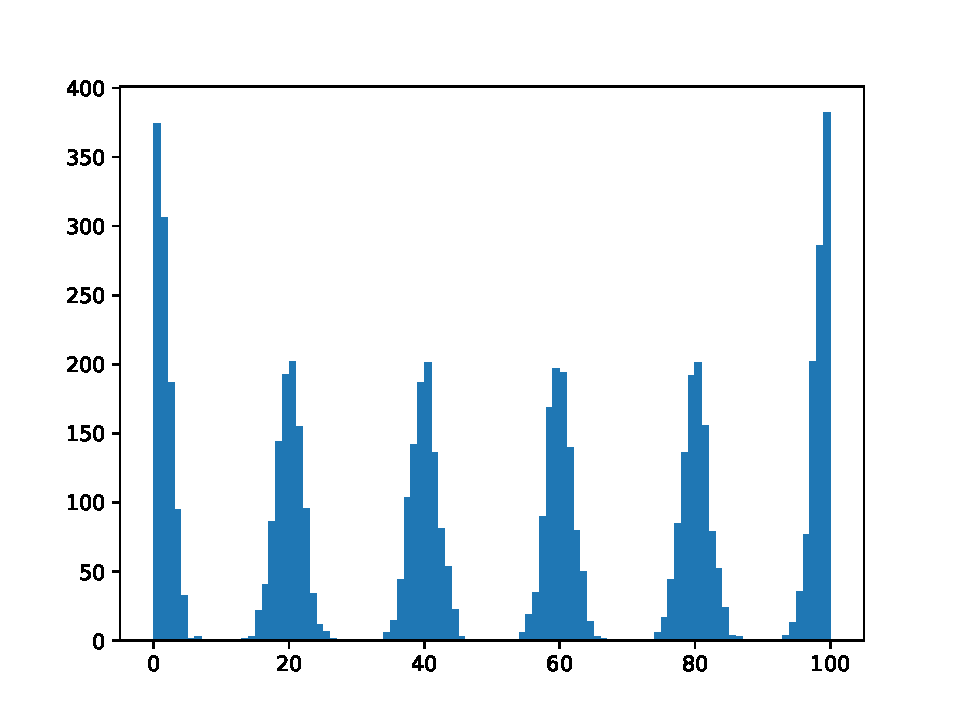
\includegraphics[width=\textwidth]{hist_2.pdf}
    \centering
    \end{subfigure}
    \begin{subfigure}[b]{0.5\textwidth}
    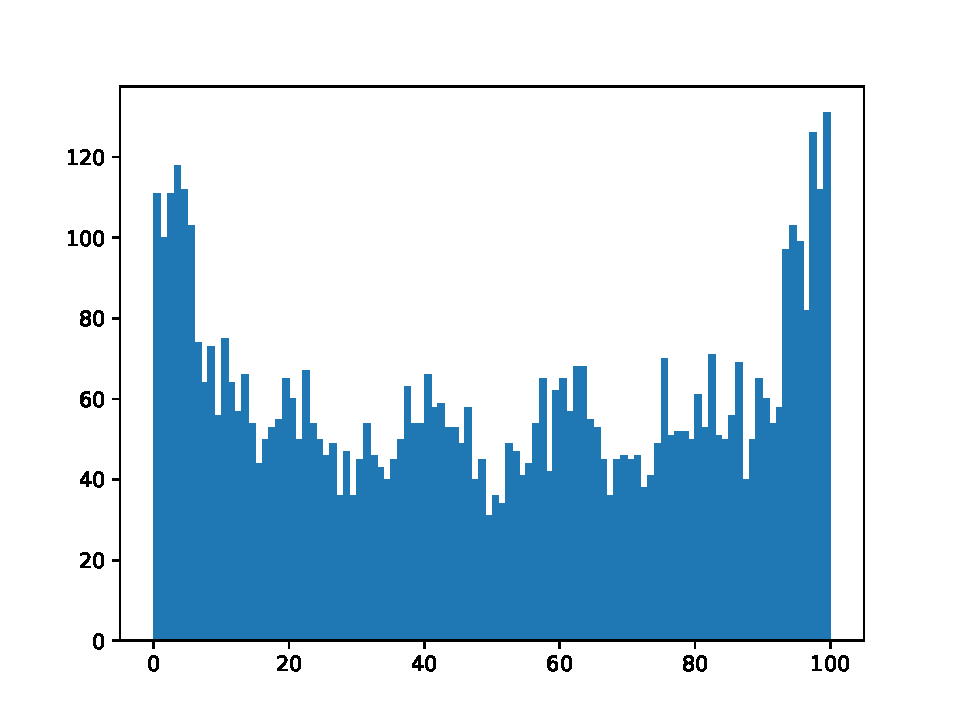
\includegraphics[width=\textwidth]{hist_7.pdf}
    \centering
    \end{subfigure}
\caption{
    Histograms of simulated counts of allele frequencies for five individuals, with differing variance.
    The x-axis shows the frequency (0\% to 100\%), and the y-axis shows how often this frequency was observed in the data.
}
\label{fig:hist}
\end{figure}

\section*{Our Questions}
\label{sec:Questions}

Given this kind of data (allele freqencies of DNA reads along the genome), we now have some questions:

\begin{enumerate}
 \item What is the noise (variance) of the observed frequencies, 
       given that we know the number of individuals in the pool?
       The straight forward approach seems to be to just cut in between the expected bins (e.g., at 10\%, 30\%, 50\%, 70\%),
       and estimate variance within each bin.
       However, maybe we can do better than this, using an ML framework, and model each frequency as a Gaussian
       (or whatever would be the appropriate distribution), and estimate parameters using a Gaussian mixture model.
       I used a simple Gaussian mixure for the histograms above for simplicity,
       that is, just combined some normal distributions. Probably, there are better multi-modal distribution to use,
       in particular when considering the boundary conditions of not allowing frequencies
       \textless 0\% or \textgreater 100\%.
       Note that for this question, we can also remove the 0\% and 100\% true frequency bins, 
       as those are ``uninteresting'' frequencies, and only consider 20\%, 40\%, 60\%, and 80\%
       as the means of the mixture components.
       This might make it easier to model, as we might just ignore the boundary conditions (unless variance is really big).
\end{enumerate}

The above is our main question. We want to use it to compare different ways of obtaining frequencies,
and quantify which of them are better (have less variance). 
In particular, we want to compare: 
(i) different biological material (Does it make a difference whether we use leaf or flower tissue of our plants?), and
(ii) different computational methods (How does our bioinformatics pipeline affect the resulting frequencies?).

Additionally, we might be interested in the following two questions, which however are not needed,
and might be hard or even impossible to tackle given the data:

\begin{enumerate}
 \setcounter{enumi}{1}
 \item Can we estimate the true frequencies? 
       This could use the same approach as whatever we figure out to use to answer the first question.
 \item Can we estimate the amount that our sequencing is off from the ideal.
       This is related to the variancethat is, but additionally, 
       can we quantify how uneven the contribution of DNA reads from each individual is?
       The Kullback-Leibler divergence might be an approach here (thanks, Julian!).
\end{enumerate}

Any hints are appreciated. There might also be more questions that are interesting in this context.

Thank you in advance, and talk to you soon \\
Lucas

\end{document}
